% -*- coding: utf-8 -*-
% Contenido del Anexo A

% Añadir al índice manualmente y asegurar anclaje correcto para hyperref
\chapter{Esquema Detallado de la Base de Datos} 
\label{app:db_schema} % Etiqueta para referenciar con \ref{}

Este anexo contiene las definiciones SQL (\texttt{CREATE TABLE}) detalladas para todas las tablas principales del sistema, incluyendo la tabla relacional \texttt{users} y las hipertablas para datos de series temporales y alertas. Se recomienda consultar la Figura~\ref{fig:esquema_relacional} para una visión global de las relaciones.

% Esquema relacional generado a partir del modelo real (ver PlantUML adjunto)
\begin{figure}[htbp]
    \centering
    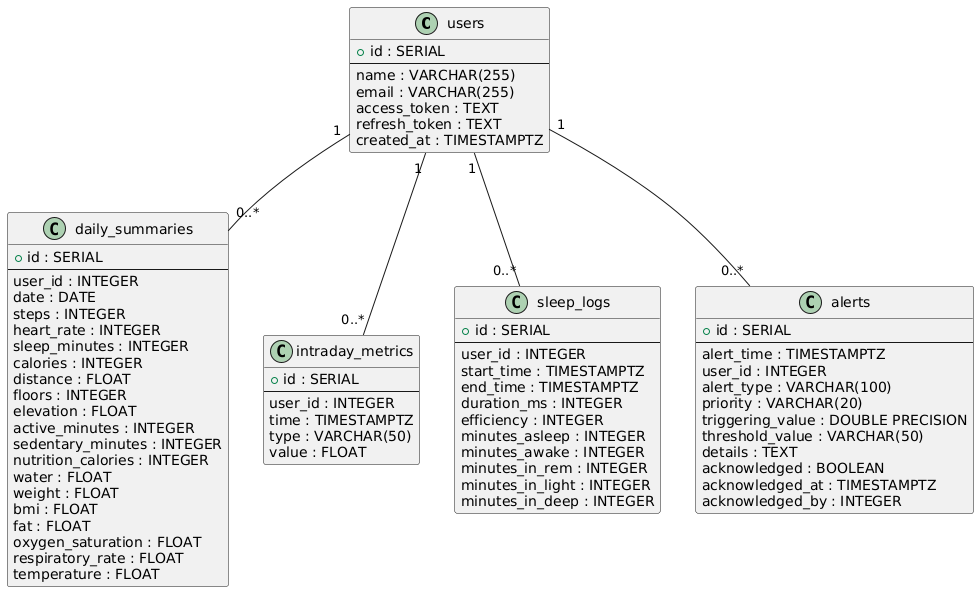
\includegraphics[width=0.9\textwidth]{imagenes/esquema_relacional.png}
    \caption{Esquema relacional de la base de datos del sistema.}
    \label{fig:esquema_relacional}
\end{figure}

\section*{Descripción de las tablas principales}
\begin{itemize}
    \item \textbf{users}: Información básica y credenciales cifradas de los usuarios.
    \item \textbf{daily\_summaries}: Resúmenes diarios de actividad, sueño y biomarcadores.
    \item \textbf{intraday\_metrics}: Datos de alta frecuencia (pasos, FC, calorías, etc.).
    \item \textbf{sleep\_logs}: Episodios de sueño detallados.
    \item \textbf{alerts}: Alertas generadas por el sistema, asociadas a usuario y condición detectada.
\end{itemize}

\section*{Tabla \texttt{users}}
Tabla relacional estándar para almacenar la información de vinculación de usuarios y credenciales cifradas.

\begin{verbatim}
CREATE TABLE IF NOT EXISTS users (
    id SERIAL PRIMARY KEY,
    name VARCHAR(255) NOT NULL,
    email VARCHAR(255) NOT NULL,
    access_token TEXT,
    refresh_token TEXT,
    created_at TIMESTAMPTZ DEFAULT CURRENT_TIMESTAMP
);
\end{verbatim}

\section*{Hipertabla \texttt{intraday\_metrics}}
Almacena datos intradía (pasos, frecuencia cardíaca, calorías, etc.) con referencia al usuario.

\begin{verbatim}
CREATE TABLE IF NOT EXISTS intraday_metrics (
    id SERIAL PRIMARY KEY,
    user_id INTEGER REFERENCES users(id),
    time TIMESTAMPTZ NOT NULL,
    type VARCHAR(50) NOT NULL,
    value FLOAT NOT NULL
);
SELECT create_hypertable('intraday_metrics', 'time', if_not_exists => TRUE, migrate_data => TRUE);
\end{verbatim}

\section*{Hipertabla \texttt{daily\_summaries}}
Almacena resúmenes diarios de actividad, sueño y biomarcadores.

\begin{verbatim}
CREATE TABLE IF NOT EXISTS daily_summaries (
    id SERIAL PRIMARY KEY,
    user_id INTEGER REFERENCES users(id),
    date DATE NOT NULL,
    steps INTEGER,
    heart_rate INTEGER,
    sleep_minutes INTEGER,
    calories INTEGER,
    distance FLOAT,
    floors INTEGER,
    elevation FLOAT,
    active_minutes INTEGER,
    sedentary_minutes INTEGER,
    nutrition_calories INTEGER,
    water FLOAT,
    weight FLOAT,
    bmi FLOAT,
    fat FLOAT,
    oxygen_saturation FLOAT,
    respiratory_rate FLOAT,
    temperature FLOAT,
    UNIQUE(user_id, date)
);
SELECT create_hypertable('daily_summaries', 'date', if_not_exists => TRUE, migrate_data => TRUE);
\end{verbatim}

\section*{Hipertabla \texttt{sleep\_logs}}
Registra episodios de sueño detallados por usuario.

\begin{verbatim}
CREATE TABLE IF NOT EXISTS sleep_logs (
    id SERIAL PRIMARY KEY,
    user_id INTEGER REFERENCES users(id),
    start_time TIMESTAMPTZ NOT NULL,
    end_time TIMESTAMPTZ NOT NULL,
    duration_ms INTEGER,
    efficiency INTEGER,
    minutes_asleep INTEGER,
    minutes_awake INTEGER,
    minutes_in_rem INTEGER,
    minutes_in_light INTEGER,
    minutes_in_deep INTEGER
);
SELECT create_hypertable('sleep_logs', 'start_time', if_not_exists => TRUE, migrate_data => TRUE);
\end{verbatim}

\section*{Hipertabla \texttt{alerts}}
Almacena las alertas generadas por el sistema, referenciando al usuario y con detalles de la condición detectada.

\begin{verbatim}
CREATE TABLE IF NOT EXISTS alerts (
    id SERIAL PRIMARY KEY,
    alert_time TIMESTAMPTZ DEFAULT CURRENT_TIMESTAMP,
    user_id INTEGER REFERENCES users(id),
    alert_type VARCHAR(100) NOT NULL,
    priority VARCHAR(20) NOT NULL,
    triggering_value DOUBLE PRECISION,
    threshold_value VARCHAR(50),
    details TEXT,
    acknowledged BOOLEAN DEFAULT FALSE
);
SELECT create_hypertable('alerts', 'alert_time', if_not_exists => TRUE, migrate_data => TRUE);
\end{verbatim}